\documentclass[12pt]{article}
\usepackage[utf8]{inputenc}
%------------------------------ tables
\usepackage{tabularx}
\usepackage{makecell}
\usepackage{amsmath} 
\usepackage{float}
%------------------------------ images
\usepackage{graphicx}
\usepackage{subcaption}

% footnotes
\setlength{\footnotesep}{0.6\baselineskip}

% Page layout
\usepackage[left=3cm,right=3cm,top=3cm,bottom=2cm]{geometry}
\setlength{\skip\footins}{2cm}

% Clickable toc and links styles
\usepackage{hyperref}
\hypersetup{
    colorlinks,
    citecolor=black,
    filecolor=black,
    linkcolor=black,
    urlcolor=blue
}
\usepackage{url}

% Title spec
\usepackage{titlesec}
\titlespacing\section{0pt}{20pt}{10pt}
\titlespacing\subsection{0pt}{15pt}{10pt}
\titlespacing\subsubsection{0pt}{10pt}{5pt}

% Page numbering and head
\usepackage{lastpage}
\usepackage{fancyhdr}
\pagestyle{fancy}
\fancyhf{}
\setlength{\headheight}{15pt}

\setlength{\parindent}{0pt}
\setlength{\parskip}{5pt}


\begin{document}

    \begin{titlepage}

        \begin{center}
        { \textit{University of Bologna} }
            \\
            \vspace{5mm}
            { \textit{Social Network Analysis} }\\
        \end{center}

        \vspace{20mm}

        \begin{center}
        {\LARGE{\textbf{Open Flights}}}
            \\
        \end{center}

        \vspace{20mm}

        \begin{center}
        {\LARGE{Analysis of OpenFlight's Airplane Routes Network}}
            \\
        \end{center}

        \vspace{30mm}

        \begin{center}
        {\large{Filippo Brajucha [0001130613]\\}}
            \vspace{5mm}
            {\large{Leonardo Dessì [0001141270] \\}}
            \vspace{5mm}
            {\large{Gianmarco Gabrielli [0001133622]  \\}}
            \vspace{5mm}
            {\large{Simone Rinaldi [0001140193]\\}}
        \end{center}

        \vspace{40mm}

    \end{titlepage}

    \tableofcontents
    \newpage


    \section{Introduction}\label{sec:introduction}
    This project falls under the specific field of \textbf{Transport Network Analysis}, an interdisciplinary research area that applies Network Science to the study of transportation systems. Transport Network Analysis uses mathematical and computational tools derived from graph theory to analyze, to model and to understand the flow of people, goods, and information through complex transportation networks.

    In this project, we apply Transport Network Analysis to the study of the global air transport system.
    Specifically, we will analyze the network of airports and the air routes that connect them to identify the most relevant and strategic airports on a global level and subsequently test the hypothesis that these airports are critical to the overall connectivity of the network.


    \section{Problem and Motivation}\label{sec:problem-and-motivation}
    The air transportation network is one of the most complex and vital networks in modern society, enabling global connectivity and supporting economic growth. Despite its importance, this network is vulnerable to disruptions caused by natural disasters, geopolitical events, technical failures, and pandemics. These disruptions can have significant cascading effects, leading to delays, economic losses, and reduced global mobility. Therefore, understanding the structure of the airline network and identifying critical nodes (airports) is crucial to ensuring the stability and resilience of air travel.

    This project aims to analyze the global network of airports and air routes.
    The main goal is to \textbf{identify the most relevant and strategic airports in terms of network}.
    \begin{itemize}
        \item Understanding the structure and dynamics of global air transport: Identifying major hubs and their influence on global connectivity can provide valuable information on how air traffic spreads around the world. This analysis can contribute to scientific research in the field of network analysis applied to air transport.
        \item Optimize route planning and air traffic management: Knowledge of the most strategic airports can help airlines optimize their routes, improving air transport efficiency and reducing costs.
        \item Improving flight network resilience to disruptions: Understanding the role of hubs in global connectivity enables assessment of the network's robustness to unforeseen events such as airport closures or route cancellations. This knowledge can be used to develop strategies that minimize the impact of such disruptions on the global air transportation system.
    \end{itemize}

    The main contributions of the project include:

    \begin{itemize}
        \item Identification of the most globally relevant airports: Using various measures of centrality such as \textit{Degree Centrality}, \textit{Eigenvector Centrality}, \textit{PageRank}, etc., the project aims to identify airports that play a key role in the global air transport network.
        \item Verification of the hypothesis that airports with high betweenness centrality are critical to global connectivity: Through robustness simulations, the project will evaluate the impact of removing these airports on network connectivity. Connectivity, fragmentation, and compactness will be used to measure the impact.
        \item The identification of regional airport clusters: Using clustering algorithms such as the community \textit{louvain algorithm}, the project will identify groups of strongly interconnected airports within specific geographic areas.
    \end{itemize}


    \section{Dataset}\label{sec:dataset}

    \subsection{Dataset Description: OpenFlights Air Route Network}\label{subsec:dataset-description:-openflights-air-route-network}
    The dataset used for this project was obtained from the \hyperlink{https://openflights.org/}{OpenFlights website} (and \hyperlink{https://github.com/jpatokal/openflights}{github}), a public resource that provides information on airports and air routes around the world.
    The data were downloaded in digital format and are freely accessible from both the website and the associated GitHub repository.
    OpenFlights data is divided into two databases:
    \begin{itemize}
        \item \textbf{Airport database}: contains information on more than 10,000 airports, train stations, and ferry terminals worldwide. Each entry includes details such as airport ID, name, city, country, IATA and ICAO codes, geographic coordinates, and data source.
        \item \textbf{Route database}: contains information on 67,663 routes among 1,578 airports, operated by 548 airlines (data as of June 2014). Each entry includes airline code, airline ID, departure airport, departure airport ID, destination airport, destination airport ID, and type of aircraft used.
    \end{itemize}
    Data manipulation and analysis tools were used to analyze and construct the airport network graph. These tools included the Python programming language, which offers libraries specifically designed for network analysis, such as NetworkX.

    The network graph used airports as nodes and direct air routes as edges. The edges were weighted according to the number of existing flights or connections between airports to reflect the intensity of air traffic.

    \subsubsection{Format and Structure}
    The process of converting the OpenFlights database into a networkX graph for network analysis is as follows:
    \begin{itemize}
        \item \textbf{Data import}: Airport and route data were imported into Python using Pandas library, which allows for the efficient handling of tabular data, enabling cleaning, filtering e formatting operation necessary to construct the air network analysis graph.
        The main step are:
             \begin{itemize}
                 \item \textbf{Data structured verification}: erroneous formats and missing or incosistent values were verified like airports with invalid IATA codes.
                 \item \textbf{Validation of Codes}: IATA and ICAO codes for airports were compared with external sources to ensure their correctness. This process helped to reduce the likelihood of errors in airport identification
             \end{itemize}
        \item \textbf{Data Cleaning}: Data cleaning was performed with the goal of removing any outliers or redundant data and ensuring that the information was an accurate and consistent as possible.
        The main cleaning of operations are:
            \begin{itemize}
                \item \textbf{Removal of duplicates}: duplicates airports or routes were removed to avoid counting the same link multiple times
                \item  \textbf{Treatment of missing data}: any missing values for airports, such as geographic coordinates, were completed where possible using reliable sources or were excluded from the analysis.
                \item \textbf{Verification of geographical congruence}: the correctness of geographical coordinates of airports was checked to avoid geographical discrepancies in route tracking
            \end{itemize}
        \item \textbf{Node creation}: Each airport in the database was converted into a graph node. Relevant information about the airport, such as name, city and country, was associated as attributes to the corresponding node.
        \item \textbf{Creation of edges}: For each air route in the database, an edge was created between the nodes corresponding to the departure and arrival airports. The presence of an edge thus indicates the existence of a direct air link between two airports.
        \item \textbf{Edge weighting}: To reflect the intensity of air traffic between airports, the arcs were weighted according to the number of flights or connections present between the two connected airports. This information was extracted from the route database and assigned as an attribute to the corresponding edge.
        \item \textbf{Distance calculation}: using the coordinates in the airport database, distances in km between each airport were calculated and added as an attribute of the edges.
        \item \textbf{Symmetrization}: in order to create an undirected graph, a summation of the weights of the edges passing through the same nodes was performed.
        The choice to symmetrize the network has implications that must be justified, especially in a context such as air traffic, where route directionality may be important. 
        We can loss the directionality information, like the information that some flights operate in particular in one direction or the impact on traffic directionality, but the use of symmetrization bring us some very important benefits.
            \begin{itemize}
                \item \textbf{Simplification of the analysis}: transforming the graph into ad undirected one, the analysis became simpler, especially in term of calculating network centrality, connectivity and robustness metrics.
                In an undirected graph, it is easier to assess how connected the airports are and which nodes are the most central.
                \item \textbf{Focus on global connectivity}: symmetrization allows the focus to be on the overall interconnectedness of the air network, highlighting which airports are crucial to maintaining connectivity globally, without having to worry about the specific direction of traffic.
            \end{itemize}
        By symmetrizing the network, the analysis shifts from the directional nature of traffic (that can be more useful and relevant in operational or management contexts) to a more global and structural view of the transportation network.
        This provide useful information like:
            \begin{itemize}
                \item \textbf{Identity major hubs}: airports with high centrality become apparent in terms of the number of global connections, regardless of traffic direction
                \item \textbf{Evaluate network robustness}: symmetrization helps identify areas of the network that are most vulnerable when nodes or arcs are removed, facilitating planning to mitigate operational risks.
            \end{itemize}
            
    \end{itemize}
    The result of this process is a weighted, undirected graph, where the nodes represent the airports and the edges represent the direct air routes between them. The weight of each edge indicates the intensity of air traffic between the connected airports.

    The structure of the graph is shown in figure~\ref{fig:graph-structure}.
    In this figure are shown only the nodes with degree greater or equal than 10, and the dimension of the node represents the betweenness centrality of the node.
    
    
    \begin{figure}[H]
        \centering
        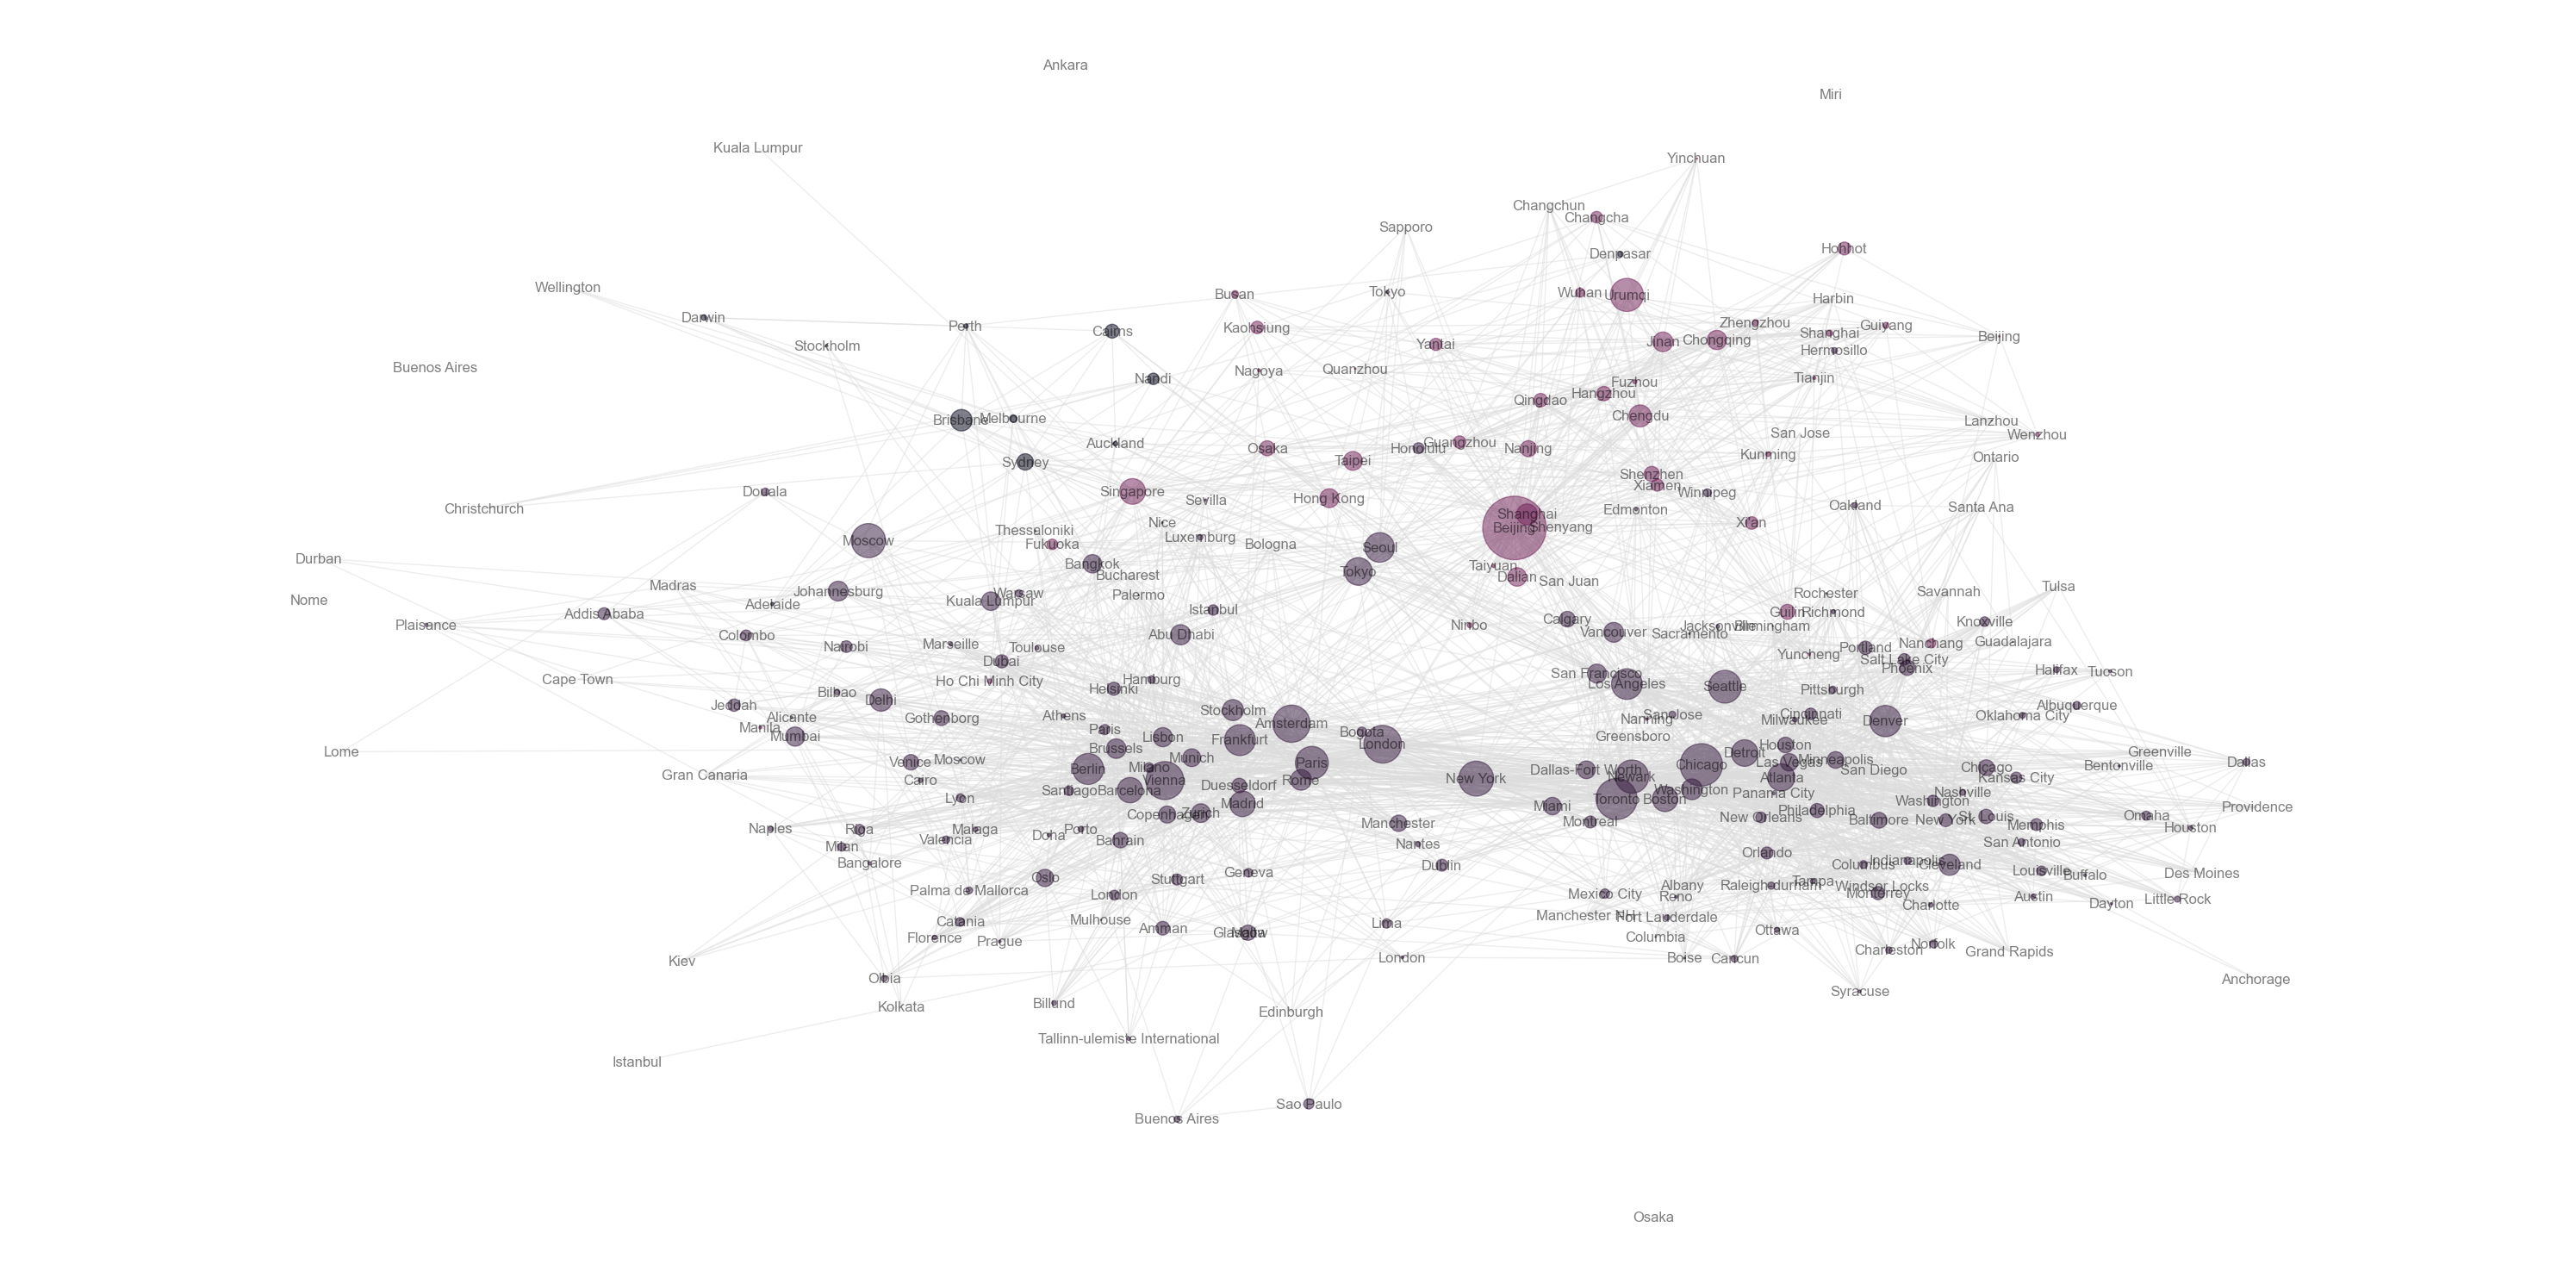
\includegraphics[width=1\linewidth]{img/graph_structure}
        \caption{Structure of the main node graph}
        \label{fig:graph-structure}
    \end{figure}

    In the figure~\ref{fig:world-graph} the nodes are placed in the world map using their coordinates, and the arcs represent the links between airports.

    \begin{figure}[H]
        \centering
        \includegraphics[width=1\linewidth]{img/graph_map_structure}
        \caption{Graph structure displayed in the world map}
        \label{fig:world-graph}
    \end{figure}

    \section{Validity and Reliability}\label{sec:validity-and-reliability}
    Our analysis is built on the reputable \texttt{OpenFlights} dataset and standard network metrics, ensuring both validity and reliability.

    To maintain validity, we:
    \begin{itemize}
        \item Use established centrality measures (e.g., degree, betweeness, eigenvector) that effectively capture airport connectivity.
        \item Construct a weighted, undirected graph that faithfully represents global air routes.
    \end{itemize}

    Reliability is ensured by:
    \begin{itemize}
        \item \textbf{Data Reliability}: The OpenFlights dataset, sourced from a reputable public repository and maintained on GitHub, is extensively used in academic research.
        This dataset was used in several and important academic studies attesting to its reliability and usefulness like:
            \begin{itemize}
                \item \textbf{\href{ https://www.nature.com/articles/srep01467}{Detecting Core-Periphery Structure in Spatial Networks}}: This study by Junteng Jia and Austin R. Benson, presented at the ACM International Conference on Web Search and Data Mining (WSDM) in 2019, uses the OpenFlights dataset to analyze core-periphery structure in spatial networks.
                \item \textbf{\href{https://www.researchgate.net/publication/289685187_Worldwide_aviation_network_vulnerability_analysis_a_complex_network_approach}{Worldwide aviation network vulnerability analysis: a complex network approach}}
                \item \textbf{Global Air Traffic Network Modeling and Analysis}:  This research uses the OpenFlights dataset to model and analyze the global air traffic network, offering insights into route density and airport centrality.
            \end{itemize}
        We have taken care to clean and preprocess the data to minimize errors and inconsistencies. Where possible, data points were cross-verified with available documentation to ensure accuracy.

        \item \textbf{Measurement Reliability}: Network metrics were computed using the established algorithms provided by the NetworkX Python library. These algorithms have been thoroughly tested in many studies, ensuring that our computations are robust. Repeating the analysis with the same dataset consistently yields identical results, confirming the reliability of the measurement process.

        \item \textbf{Replicability}: We have provided a detailed description of our methodology, from data import and preprocessing to network construction and metric computation. The use of open-source tools such as Python, Pandas, and NetworkX ensures that other researchers can replicate our analysis under similar conditions. This transparency in our workflow enhances the replicability of the study.

        \item \textbf{Sensitivity Analysis}: To further assess reliability, we conducted robustness tests by removing the top hub nodes and evaluating the impact on network fragmentation and compactness.
        The observed changes were consistent with theoretical expectations, demonstrating that the network's behavior under stress aligns with our computed metrics.
        Such sensitivity analysis lends additional support to the reliability of our results.

    \end{itemize}

    Despite the rigorous approach, certain limitations must be acknowledged. The dataset represents a static snapshot of the air transportation network and may not capture temporal dynamics or recent changes in air traffic. Additionally, the decision to symmetrize the graph, while useful for the analysis, may result in the loss of directional information that could be significant in other contexts.

    


    \section{Measures and Results}\label{sec:measures-and-results}
    For the metrics graph we use the \texttt{IATA/FAA} value id, in order to distinguish every airport. It's important to say that there could be more than 1 airport in the same city.

    \subsection{Measures}\label{subsec:measures}
    This dataset is ideal for exploring various network science topics, including:
    \begin{itemize}
        \item \textbf{Degree Centrality}: Evaluate the relative importance of a node based on the number of direct connections it has. Airports with high degree centrality are those that serve as primary points of connectivity in the network by offering a larger number of direct flights to different destinations. This high connectivity makes them essential to the efficiency and accessibility of the overall air transportation network.
        \item \textbf{Betweenness Centrality}: Quantifies the extent to which a particular node serves as a bridge or intermediary in the network. In the context of air travel, it measures how frequently an airport lies on the shortest paths between other pairs of airports
        \item \textbf{Closeness Centrality}: It measures the average shortest path distance from a given airport to all other airports. Airports with high closeness centrality are those that can quickly reach, or be reached by, other airports in the network, making them strategically helpful for minimizing travel time and improving accessibility.
        \item \textbf{Eigenvector Centrality}: Measures how well-connected an airport is to others. An airport with high eigenvector centrality is one that not only has many connections but is also linked to other highly connected and influential hubs, amplifying its importance within the global air transportation network.
        \item \textbf{PageRank}: It evaluates the significance of an airport by considering not only the number of its connections but also the importance of the airports it is connected to. This metric highlights influential airports, even when many of their connections are to less prominent nodes.
        \item \textbf{Clustering Coefficient}: Quantifies how likely it is that an airport's neighboring airports (i.e., those directly connected to it) are also connected to one another. It provides insights into the local interconnectedness of an airport's surrounding network.
        \item \textbf{K-core}: Identifies a subnetwork of airports that are highly interconnected, where each airport in the subnetwork has at least k connections to other airports in that subnetwork. The k-core helps to highlight core airports that are central to a more tightly-knit cluster of airports within the broader network.
    \end{itemize}

    \subsection{Results}\label{subsec:results}

    \subsubsection{Degree Centrality}
    This chart shows the top 10 airports ranked by their degree centrality, which measures the number of direct connections an airport has with others. We can see as cities such as \textbf{Atlanta} (ATL) and \textbf{Chicago} (ORD) has a degree centrality value much higher than others (almost higher than \textit{0.09}), starting from \textbf{Denver} (DEN) the value descent, it remains on \textit{0.07} for all the top 13 airports and then it falls under \textit{0.06}.\\
    Their high-degree values indicate that these urban centers serve as major direct connectivity hubs.\\
    We can make some observation linked to the macro-areas represented by the continents.\\
    It's curious to see that the top 3 (also top 4) is totally composed by US cities, so we can assume the centrality of this state in direct airplane connection across the World, there are other US cites in the top 10.\\
    Looking at european cities we can see that in the top 10 there is \textbf{Vienna} (VIE), \textbf{London} (LHR), \textbf{Paris} (CDG) and \textbf{Amsterdam} (AMS).\\
    It's also curious to see that there is just 1 asian city in the top 10 rank, \textbf{Beijing} (PEK). We can imagine that there could be some problems linked to a "bottleneck effect" with just 1 city with high degree centrality.

    \begin{figure}[H]
        \centering
        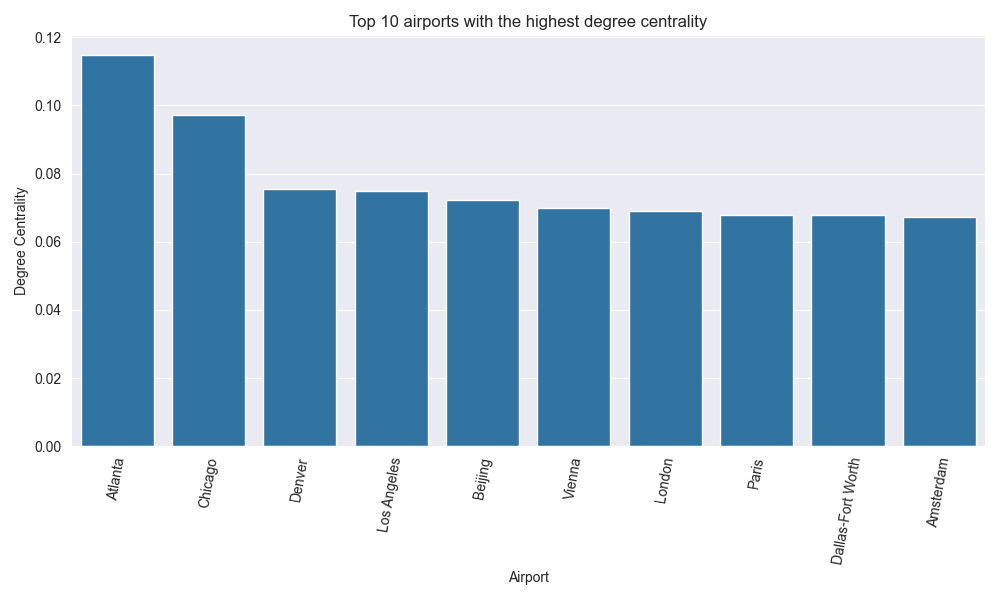
\includegraphics[width=0.8\linewidth]{img/degree_centrality.png}
    \end{figure}

    \subsubsection{Betweenness Centrality}
    This bar chart shows the top 10 airports with the highest betweenness centrality. \\
    Cities like \textbf{Dallas} (DFW) and \textbf{Beijing} (PEK) rank highest in betweenness centrality. This suggests that they play a key role as intermediaries, facilitating indirect connections across the network.\\
    We can find a lot of cities that appears in between centrality top 10 and also in degree centrality, this suggests that these nodes are the main controller of the airplane flow. These cities are very strong bridges that allow the connection across the World.\\
    The first 5 cities (Dallas, Beijing, Amsterdam, Los Angeles LAX and Singapore SIN) have little higher value than others, so we can assume that are more important. It's fascinating how there are 2 asian cities that have not so high degree centrality but high betweenness centrality.

    \begin{figure}[H]
        \centering
        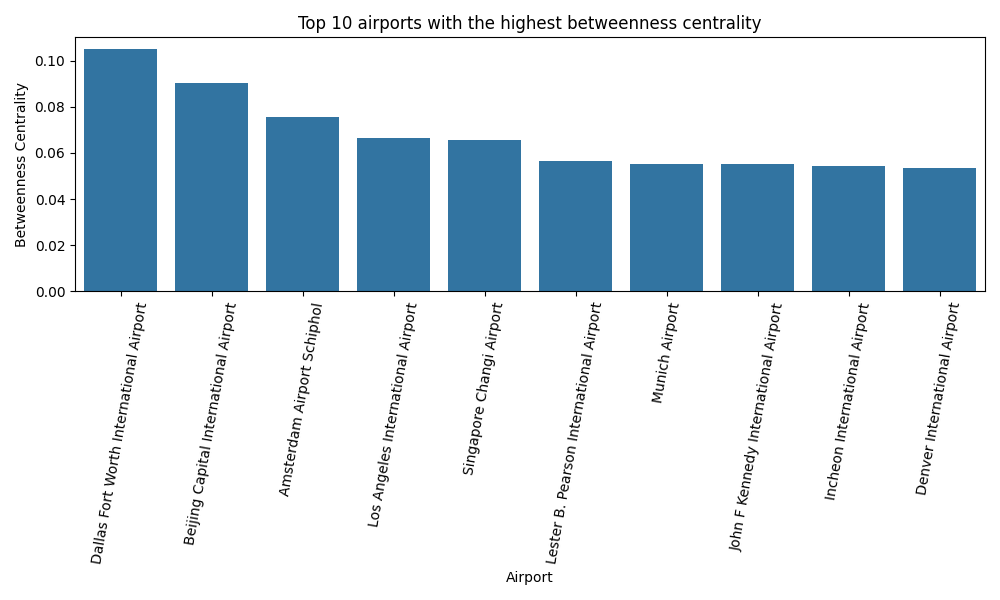
\includegraphics[width=0.8\linewidth]{img/betweenness_centrality}
    \end{figure}

    \subsubsection{Closeness Centrality}
    This chart ranks the top 10 airports according to closeness centrality, a measure of how well-connected an airport is within the network. High closeness means a node can quickly reach all other nodes, making it efficient for information spread.\\
    It's not really self-explanatory because the value is stable for a lot of airport around \texttt{0.00012}, but we can assume that the network is well-connected.\\
    We also plot the result with more than 20 airports.

    \begin{figure}[H]
        \centering
        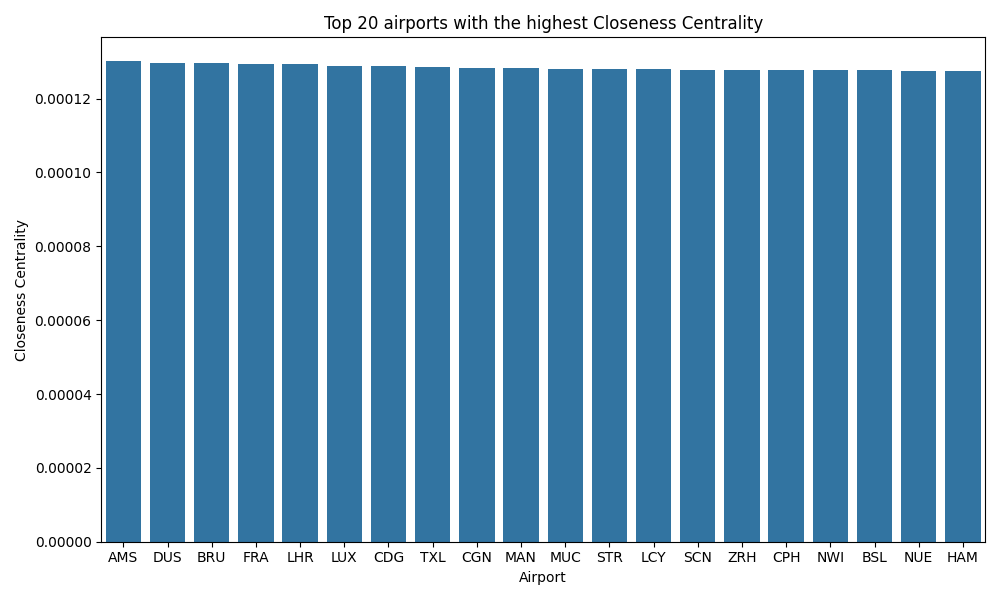
\includegraphics[width=0.8\linewidth]{img/closeness_centrality}
    \end{figure}
    \begin{figure}[H]
        \centering
        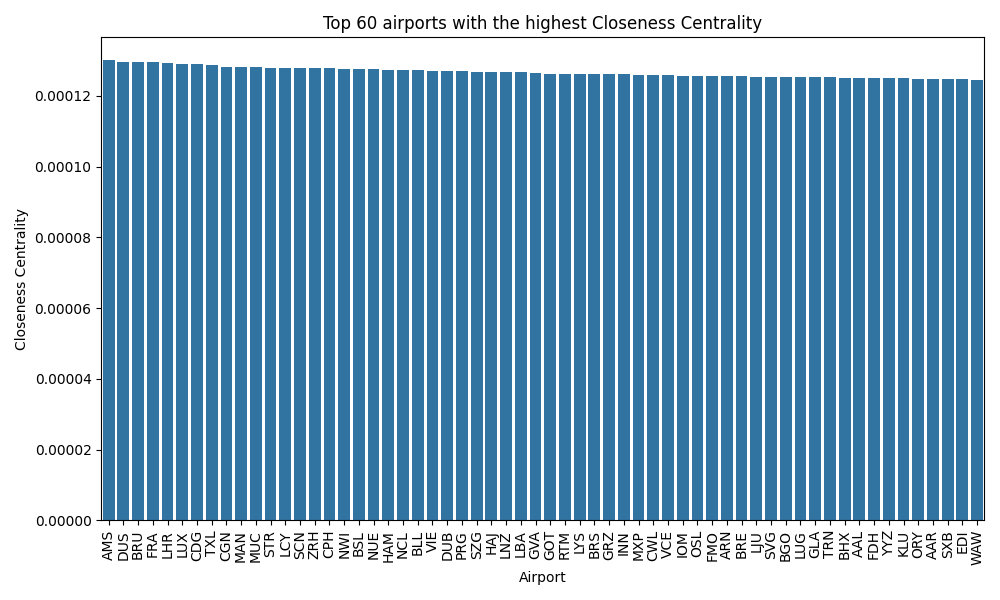
\includegraphics[width=0.8\linewidth]{img/more_closeness_centrality}
    \end{figure}

    It is important to clarify that in the context of airports, “closeness centrality” does not refer primarily to the dissemination of digital information, but rather to the ease of physical movement of passengers, cargo and aircraft. Although there are instant communication methods for information, physical transportation remains essential for people and cargo.

    “Closeness centrality” captures the efficiency of the air transportation network in minimizing physical distances and travel time. An airport with high “closeness centrality” is beneficial not because it disseminates information faster, but because it facilitates more efficient movement through the physical network. In other words, it minimizes the effort required to “travel” through the network, where “travel” refers to the movement of passengers and cargo.
    
    In summary, “closeness centrality” in the airport context is a measure of the efficiency with which airports are interconnected, facilitating faster and more accessible transportation, and is not directly related to digital information dissemination.

    \subsubsection{Clustering Coefficient}
    This bar chart shows the top 20 airports by clustering coefficient, suggesting they maintain tightly-knit local neighborhoods where many neighboring cities are also directly connected. Chiang Mai International Airport (CNX) leads with a coefficient of \texttt{0.18}, followed by Austin (GRB) with \texttt{0.17} and Fort Smith (FSM) and James City (EWN) with around \texttt{0.15}. The values decrease gradually to \texttt{0.125} for Jacksonville Airport (OAJ). These airports serve as local hubs where connected airports also tend to connect with each other.\\
    It's interesting to see that there are littler american airports than the bigger ones, it means that the USA has a well-connected structure of internal flights in order to move across different states.

    \begin{figure}[H]
        \centering
        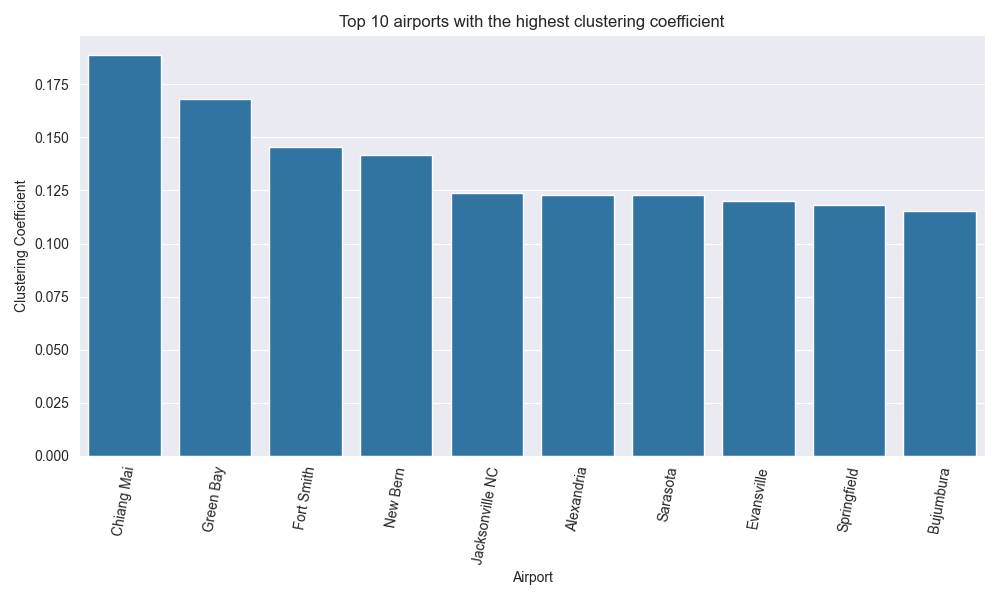
\includegraphics[width=0.8\linewidth]{img/clustering_coefficient}
    \end{figure}

    \subsubsection{K-cores}
    K-Cores are used to identify the most tightly connected parts of a graph and can provide insights into the overall structure and behavior of a network. Here we can see that the 20 airports with the highest core number is equal to 16.\\
    Because of the nature of the metrics we decided to see the others airport that has k-cores equal to 16 so we plotted other results. As we can see they are more than 50. So the network analyzed has a robust core group made by at least 50 airports across the world.

    \begin{figure}[H]
        \centering
        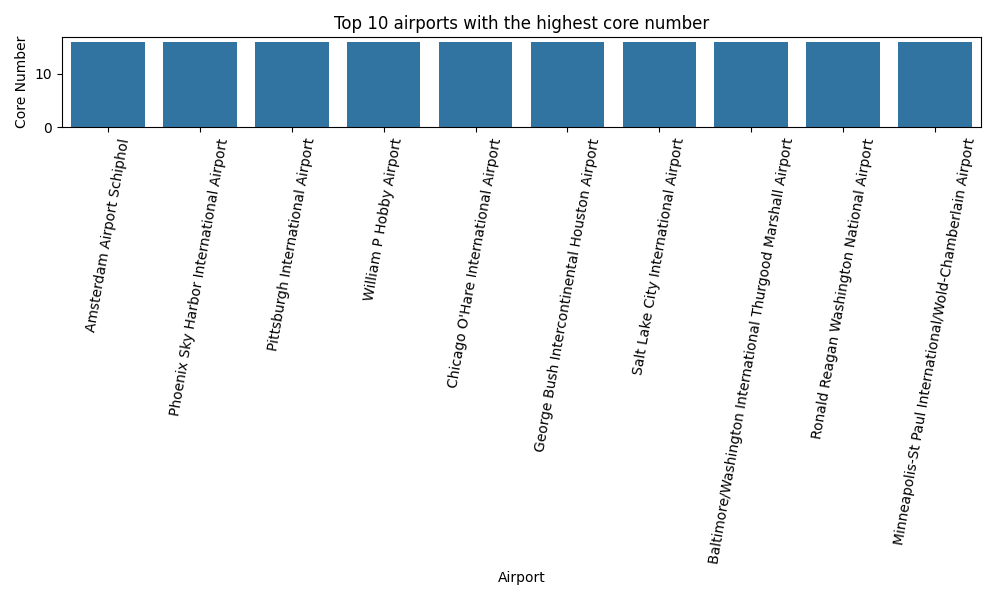
\includegraphics[width=0.8\linewidth]{img/core_number}
    \end{figure}
    \begin{figure}[H]
        \centering
        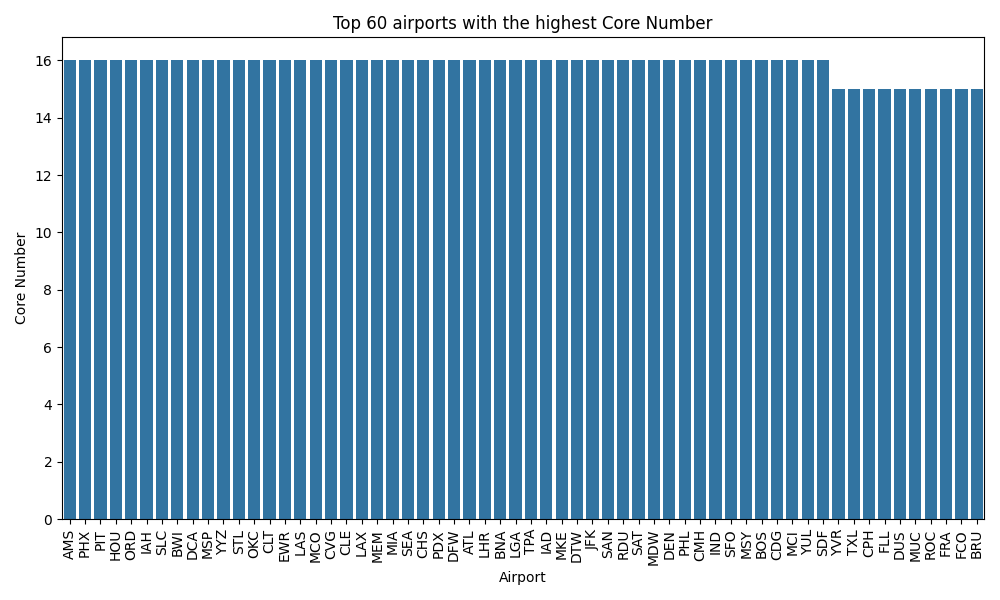
\includegraphics[width=0.8\linewidth]{img/more_core_number}
    \end{figure}

    \textbf{Definition and calculation of small-worldness}\
        Small-worldness $\sigma$ is a quantitative measure that determines how much a network behaves as a "small-world network," comparing its properties with those of an equivalent random graph. In our code, it is calculated using the NetworkX function \texttt{nx.algorithms.smallworld.sigma()}:
        \begin{verbatim}
        small_worldness = nx.algorithms.smallworld.sigma(OF_graph, niter=1, nrand=2)
        \end{verbatim}
        This function calculates the parameter $\sigma$ according to the formula:
        \begin{equation}
            \sigma = \frac{C/C_{\text{rand}}}{L/L_{\text{rand}}}
        \end{equation}
        Where:
        \begin{itemize}
        \item C is the average clustering coefficient of the real network
        \item C{rand} is the average clustering coefficient of an equivalent random network
        \item L is the average shortest path length of the real network
        \item L{rand} is the average shortest path length of an equivalent random network
        \end{itemize}
        \textbf{Interpretation in the context of air transport networks}
        In the context of the OpenFlights air transport network, a small-worldness value $\sigma$ > 1 indicates that:
        \begin{itemize}
        \item \textbf{High local clustering}: Airports tend to form densely connected regional communities (e.g., national hubs with numerous internal connections)
        \item \textbf{Short global paths}: Despite the presence of these regional clusters, it is possible to reach any airport in the network with a relatively low number of flights (typically 3-4 stopovers)
        \end{itemize}
        An air transport network with small-world properties thus shows the coexistence of two seemingly contradictory phenomena: strong local grouping and short global distances.\
        \textbf{Relevance for transport network analysis}\
        The analysis of small-worldness in air transport networks is particularly relevant for:
        \begin{itemize}
        \item \textbf{Network resilience}: Small-world networks are generally robust against random failures (random airport closures), but vulnerable to targeted attacks on main hubs
        \item \textbf{Operational efficiency}: Small-world networks facilitate rapid transfers of passengers and goods, minimizing the number of necessary stopovers
        \item \textbf{Propagation of phenomena}: Modeling how delays, cancellations, or even epidemics can rapidly propagate through the network
        \item \textbf{Network development}: Understanding how the strategic addition of new routes can improve global connectivity
        \end{itemize}
        \textbf{Output in the analyzed code}\
        In our code, the function \texttt{sigma()} produces a numerical value that is then interpreted:
        \begin{verbatim}
        print(f'small worldness: {small_worldness}')
        if small_worldness > 1:
        print("The network is a small-world network.")
        else:
        print("The network is not a small-world network.")
        \end{verbatim}
        The parameters \texttt{niter=1} and \texttt{nrand=2} in the function call indicate:
        \begin{itemize}
        \item \texttt{niter}: Number of iterations for the calculation (ideally should be increased for more robust results)
        \item \texttt{nrand}: Number of random networks generated for comparison (this should also be increased in a rigorous analysis)
        \end{itemize}
        \textbf{Limitations and methodological considerations}\
        It is also important to highlight some limitations of the approach:
        \begin{itemize}
        \item The low values of \texttt{niter} and \texttt{nrand} in the code may produce unreliable estimates of $\sigma$. For a rigorous analysis, higher values (e.g., niter=10, nrand=10) would be advisable.
        \item The small-world property is influenced by the size of the network and its density. It is useful to compare the value of $\sigma$ with other transport networks of similar size.
        \item The symmetrization of the network (transforming directional links into non-directional ones) might affect the interpretation, as in reality not all air routes are bidirectional.
        \item The calculation only considers the topology of the network and does not take into account factors such as flight capacity, frequency, or seasonality of routes.
        \end{itemize}

    \begin{figure}[H]
        \centering
        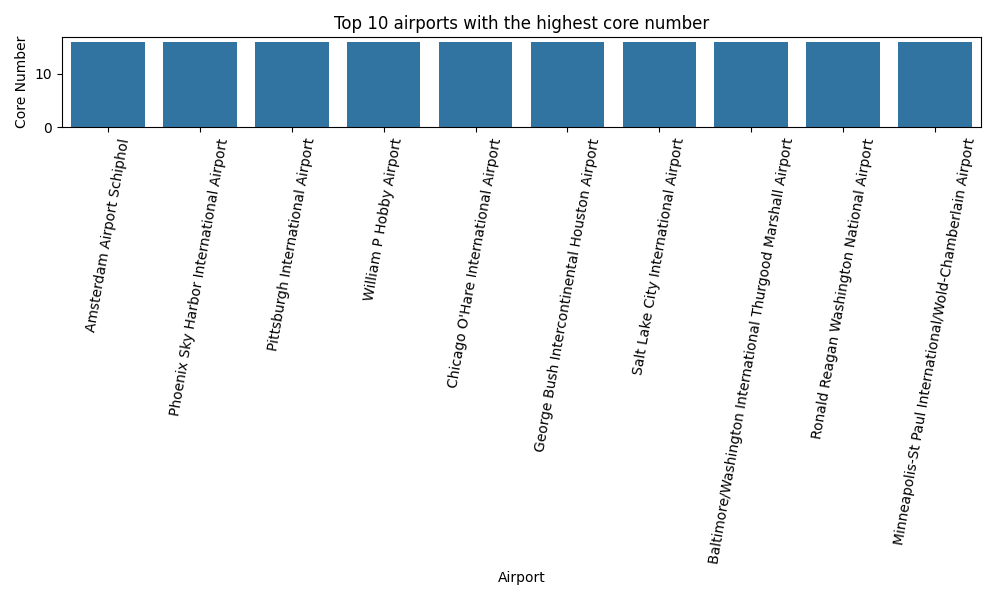
\includegraphics[width=0.8\linewidth]{img/core_number}
    \end{figure}
    \begin{figure}[H]
        \centering
        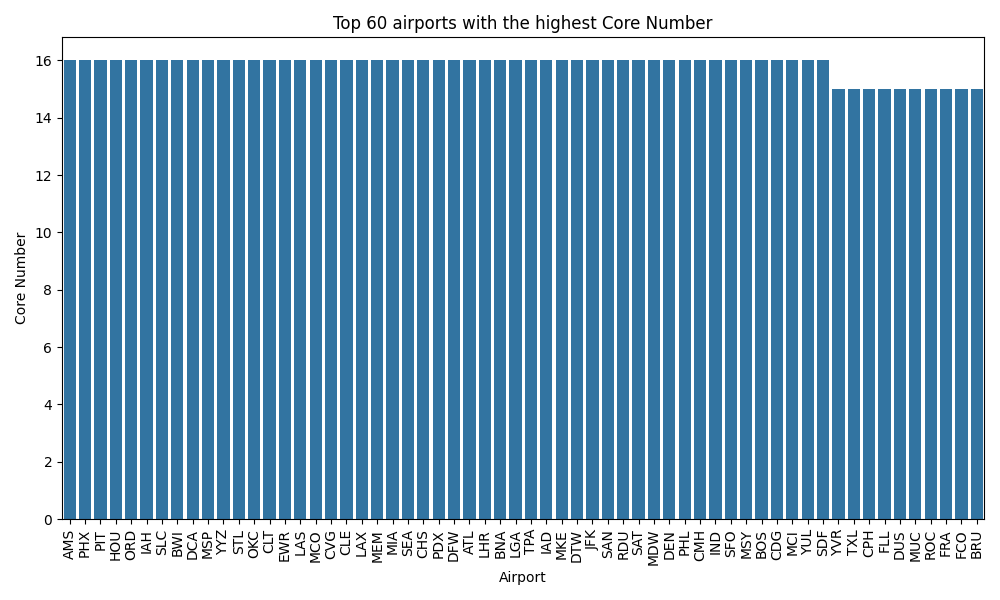
\includegraphics[width=0.8\linewidth]{img/more_core_number}
    \end{figure}
    

    \subsubsection{Eigenvector Centrality}
    The rankings again favor influential hubs such as \textbf{Atlanta} (ATL) and \textbf{Chicago} (ORD). Their high scores reflect not only many connections but also links to other highly connected cities. An airport with many connections to small, isolated airports would have a lower eigenvector centrality than one with fewer connections to major hubs.\\
    We can see that the first 2 position are occupied by the same airport that has also high Degree Centrality, so we can assume that they are crucial for the network and they could represent a \textit{bottleneck} in the network.\\    

    \begin{figure}[H]
        \centering
        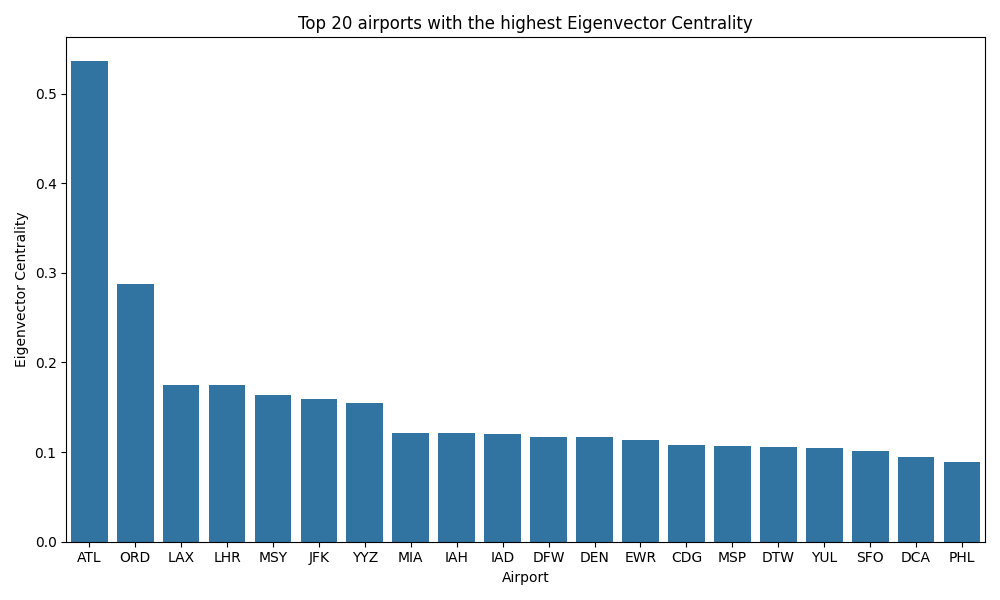
\includegraphics[width=0.8\linewidth]{img/eigenvector_centrality}
    \end{figure}

    \subsubsection{Pagerank}
    Results mirror those of eigenvector centrality, with cities like \textbf{Atlanta} (ATL), \textbf{Chicago} (ORD), and \textbf{Los Angeles} (LAX) emerging as pivotal nodes. This metric emphasizes the importance of quality as well as quantity in their connections.\\
    This metric is also very similar to the Eigenvector ones because of it's nature, but it evidence better the importance of ATL airport.
    
    \begin{figure}[H]
        \centering
        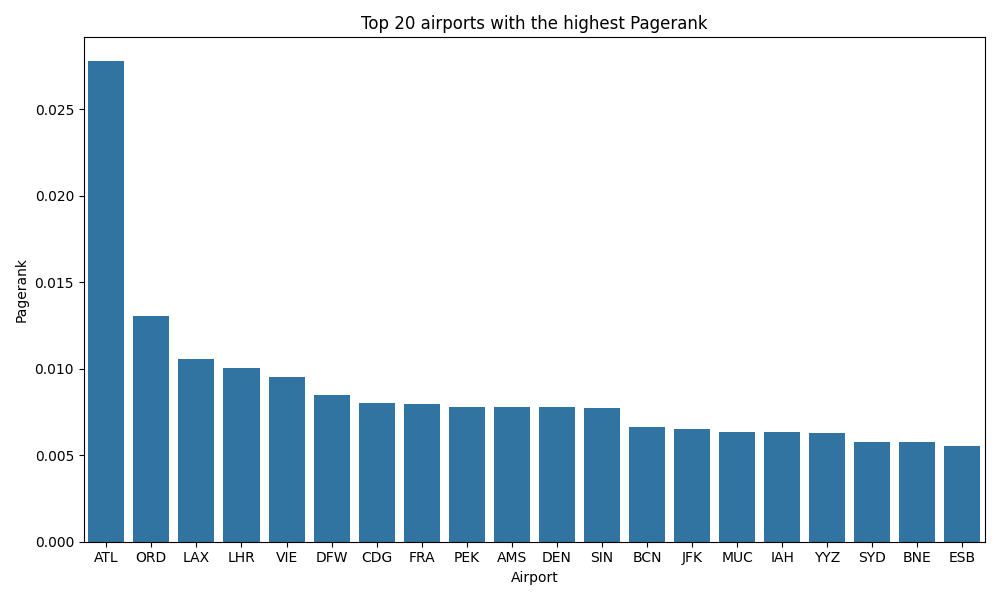
\includegraphics[width=0.8\linewidth]{img/pagerank}
    \end{figure}

    \subsubsection{Metrics distribution}
    In the following figures are displayed node metric distributions in both linear and log scales. The linear scale clearly shows absolute differences and the overall spread of values across the network. However, many network metrics, such as degree or centrality measures, tend to be highly skewed or follow a heavy-tailed distribution. A log scale compresses the high-end values and expands the lower end, making it easier to observe patterns in the tail (e.g., power-law behavior) and identify significant yet less frequent nodes. Together, these views provide a more complete understanding of the network's structure.
    \begin{figure}[H]
        \centering
        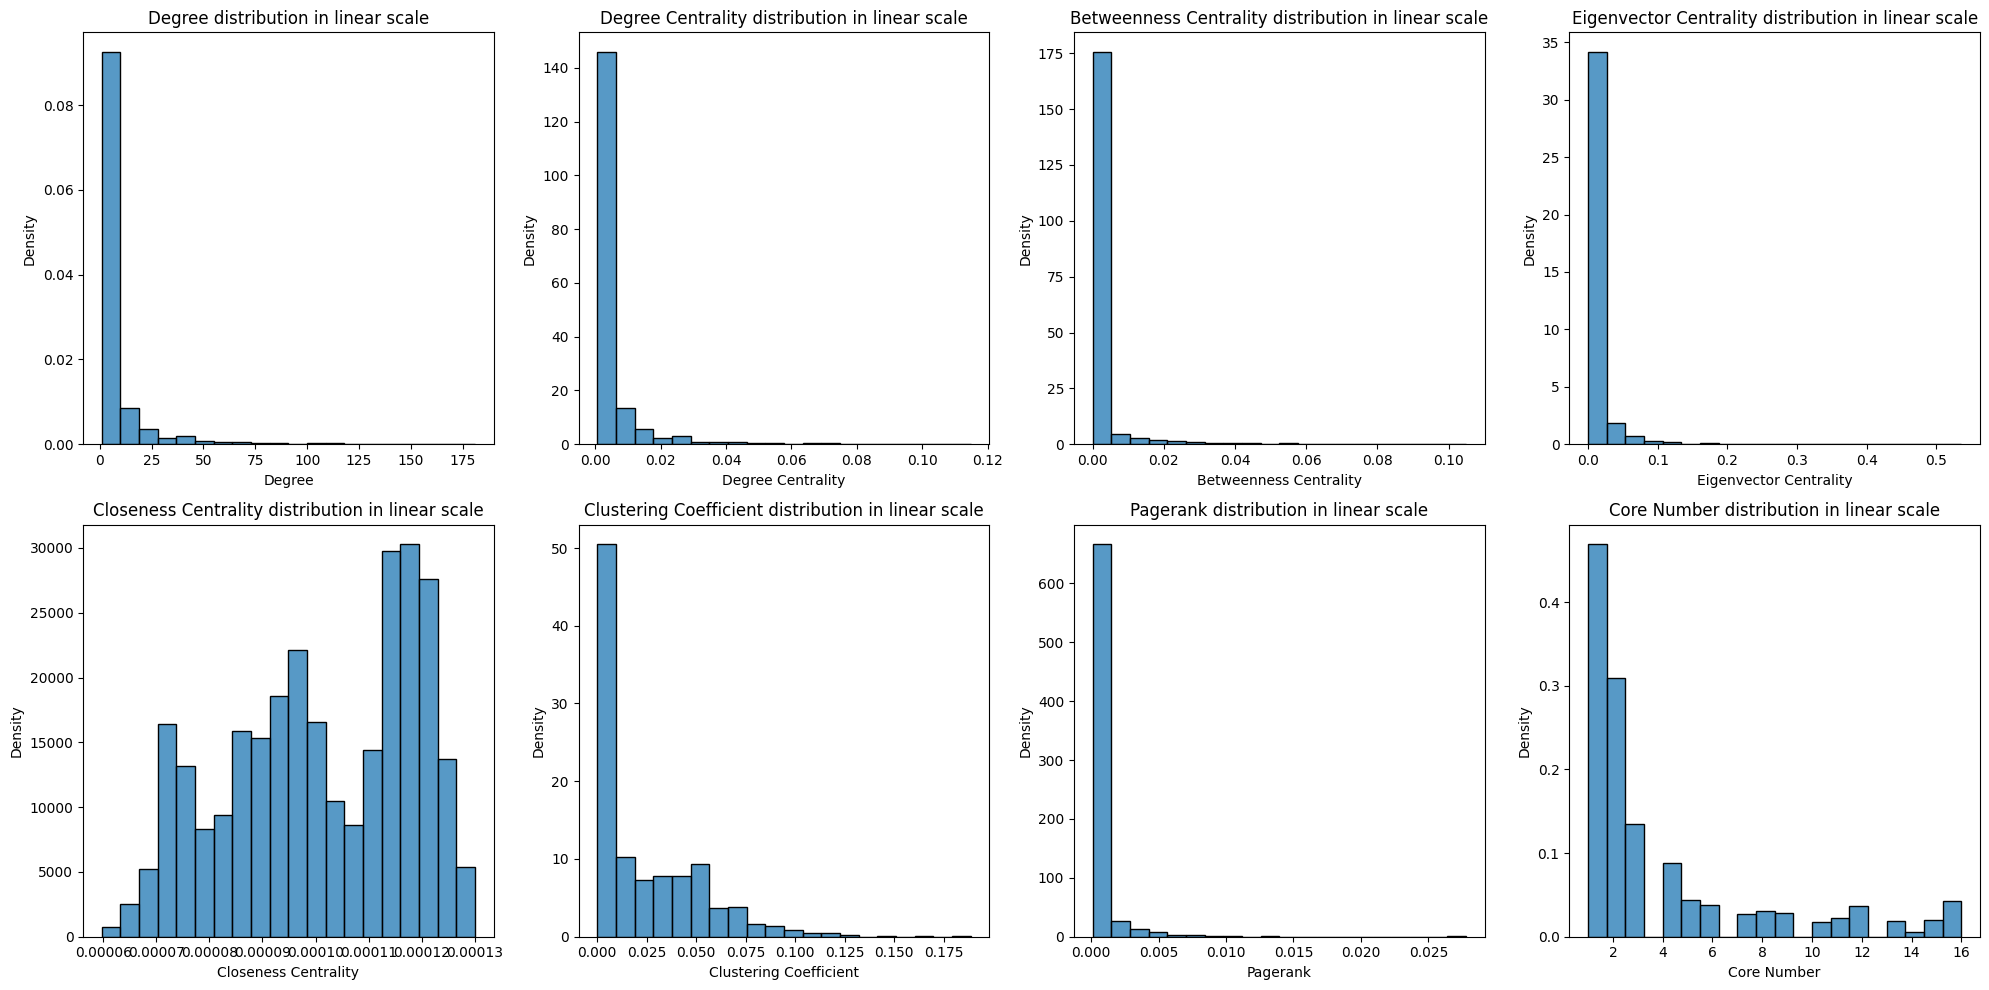
\includegraphics[width=0.8\linewidth]{img/metrics_output}
        \caption{Metrics distribution in linear-scale}
    \end{figure}

    \begin{figure}[H]
        \centering
        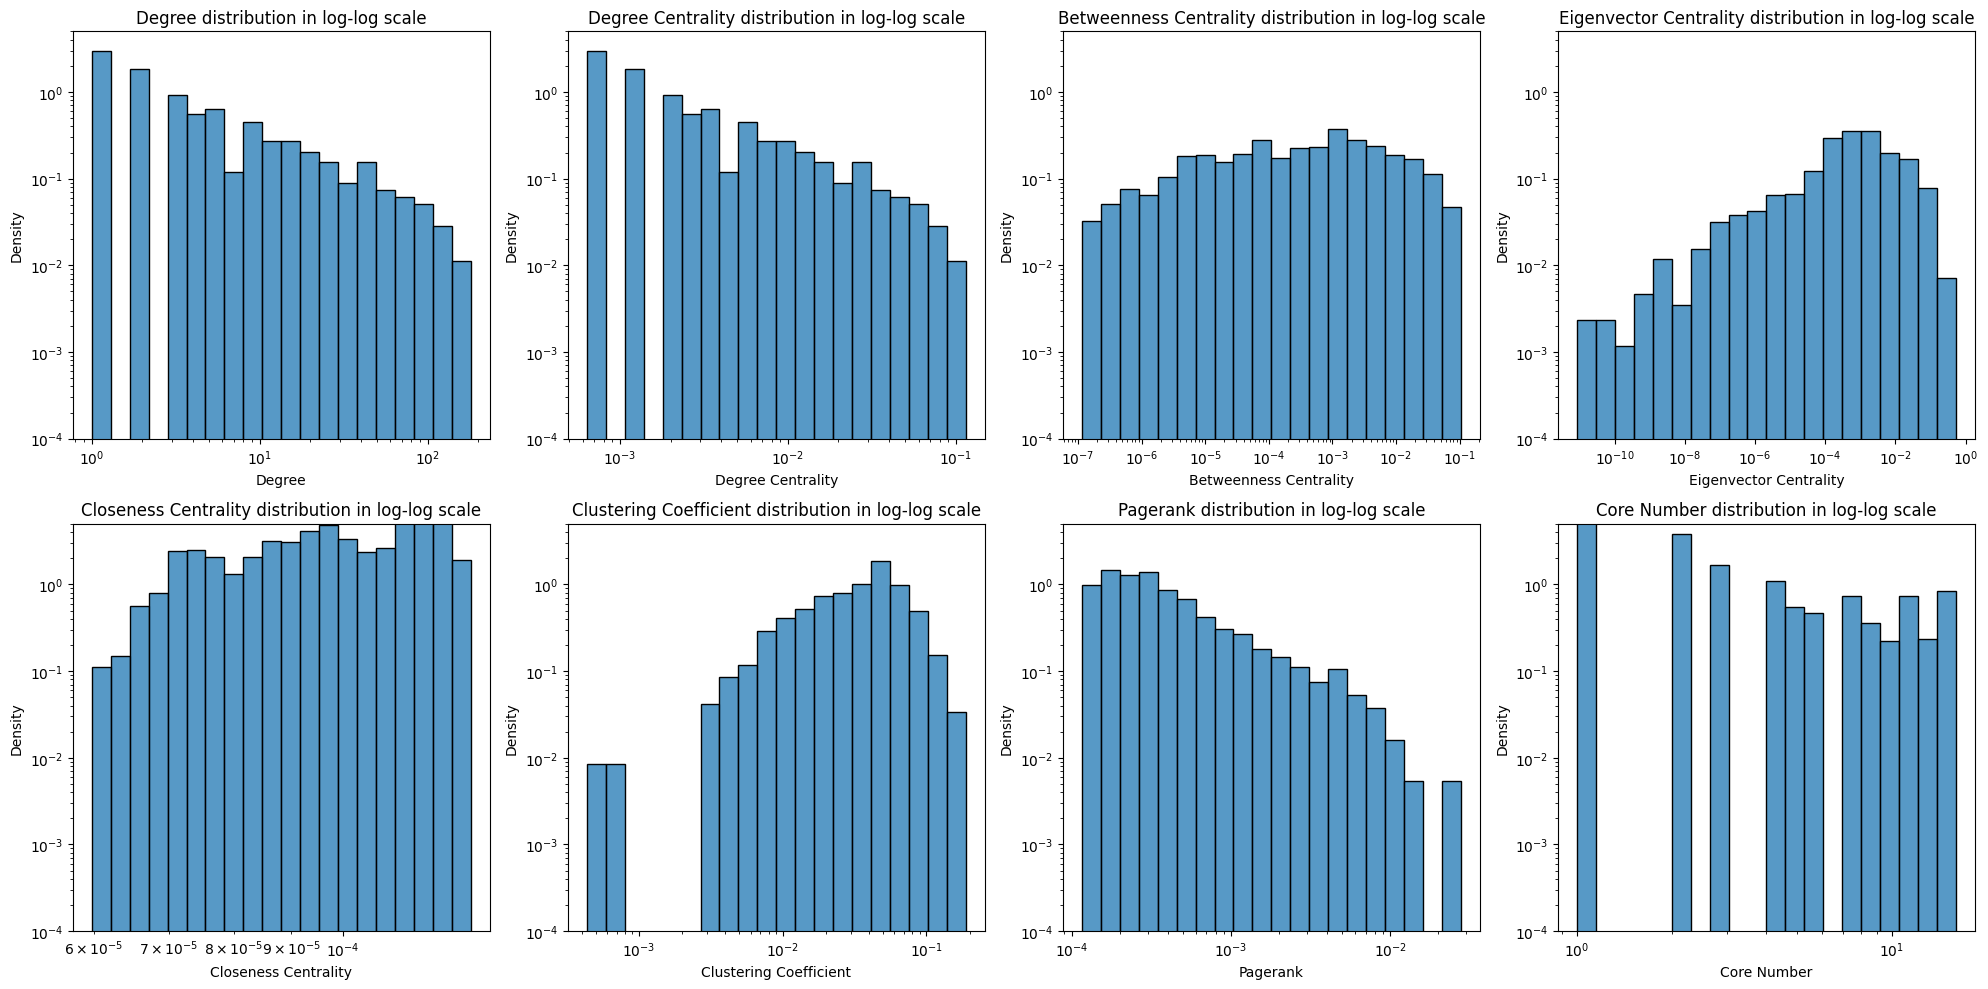
\includegraphics[width=0.8\linewidth]{img/metrics_logscale_output}
        \caption{Metrics distribution in log-scale}
    \end{figure}

    \subsubsection{Density}
    The computed density of \texttt{4.57e-3} indicates that only about \texttt{0.46\%} of all possible connections between airports are present in the network. This very low density is expected in an air transport network, where airports are not universally connected but rather linked through a few strategic routes and major hubs. The sparsity highlights that the network relies on selective connectivity to maintain efficiency and manage logistical constraints, rather than having a fully connected structure.

    \subsection{Analysis of Distribution Queues}
    \begin{figure}[H]
        \centering
        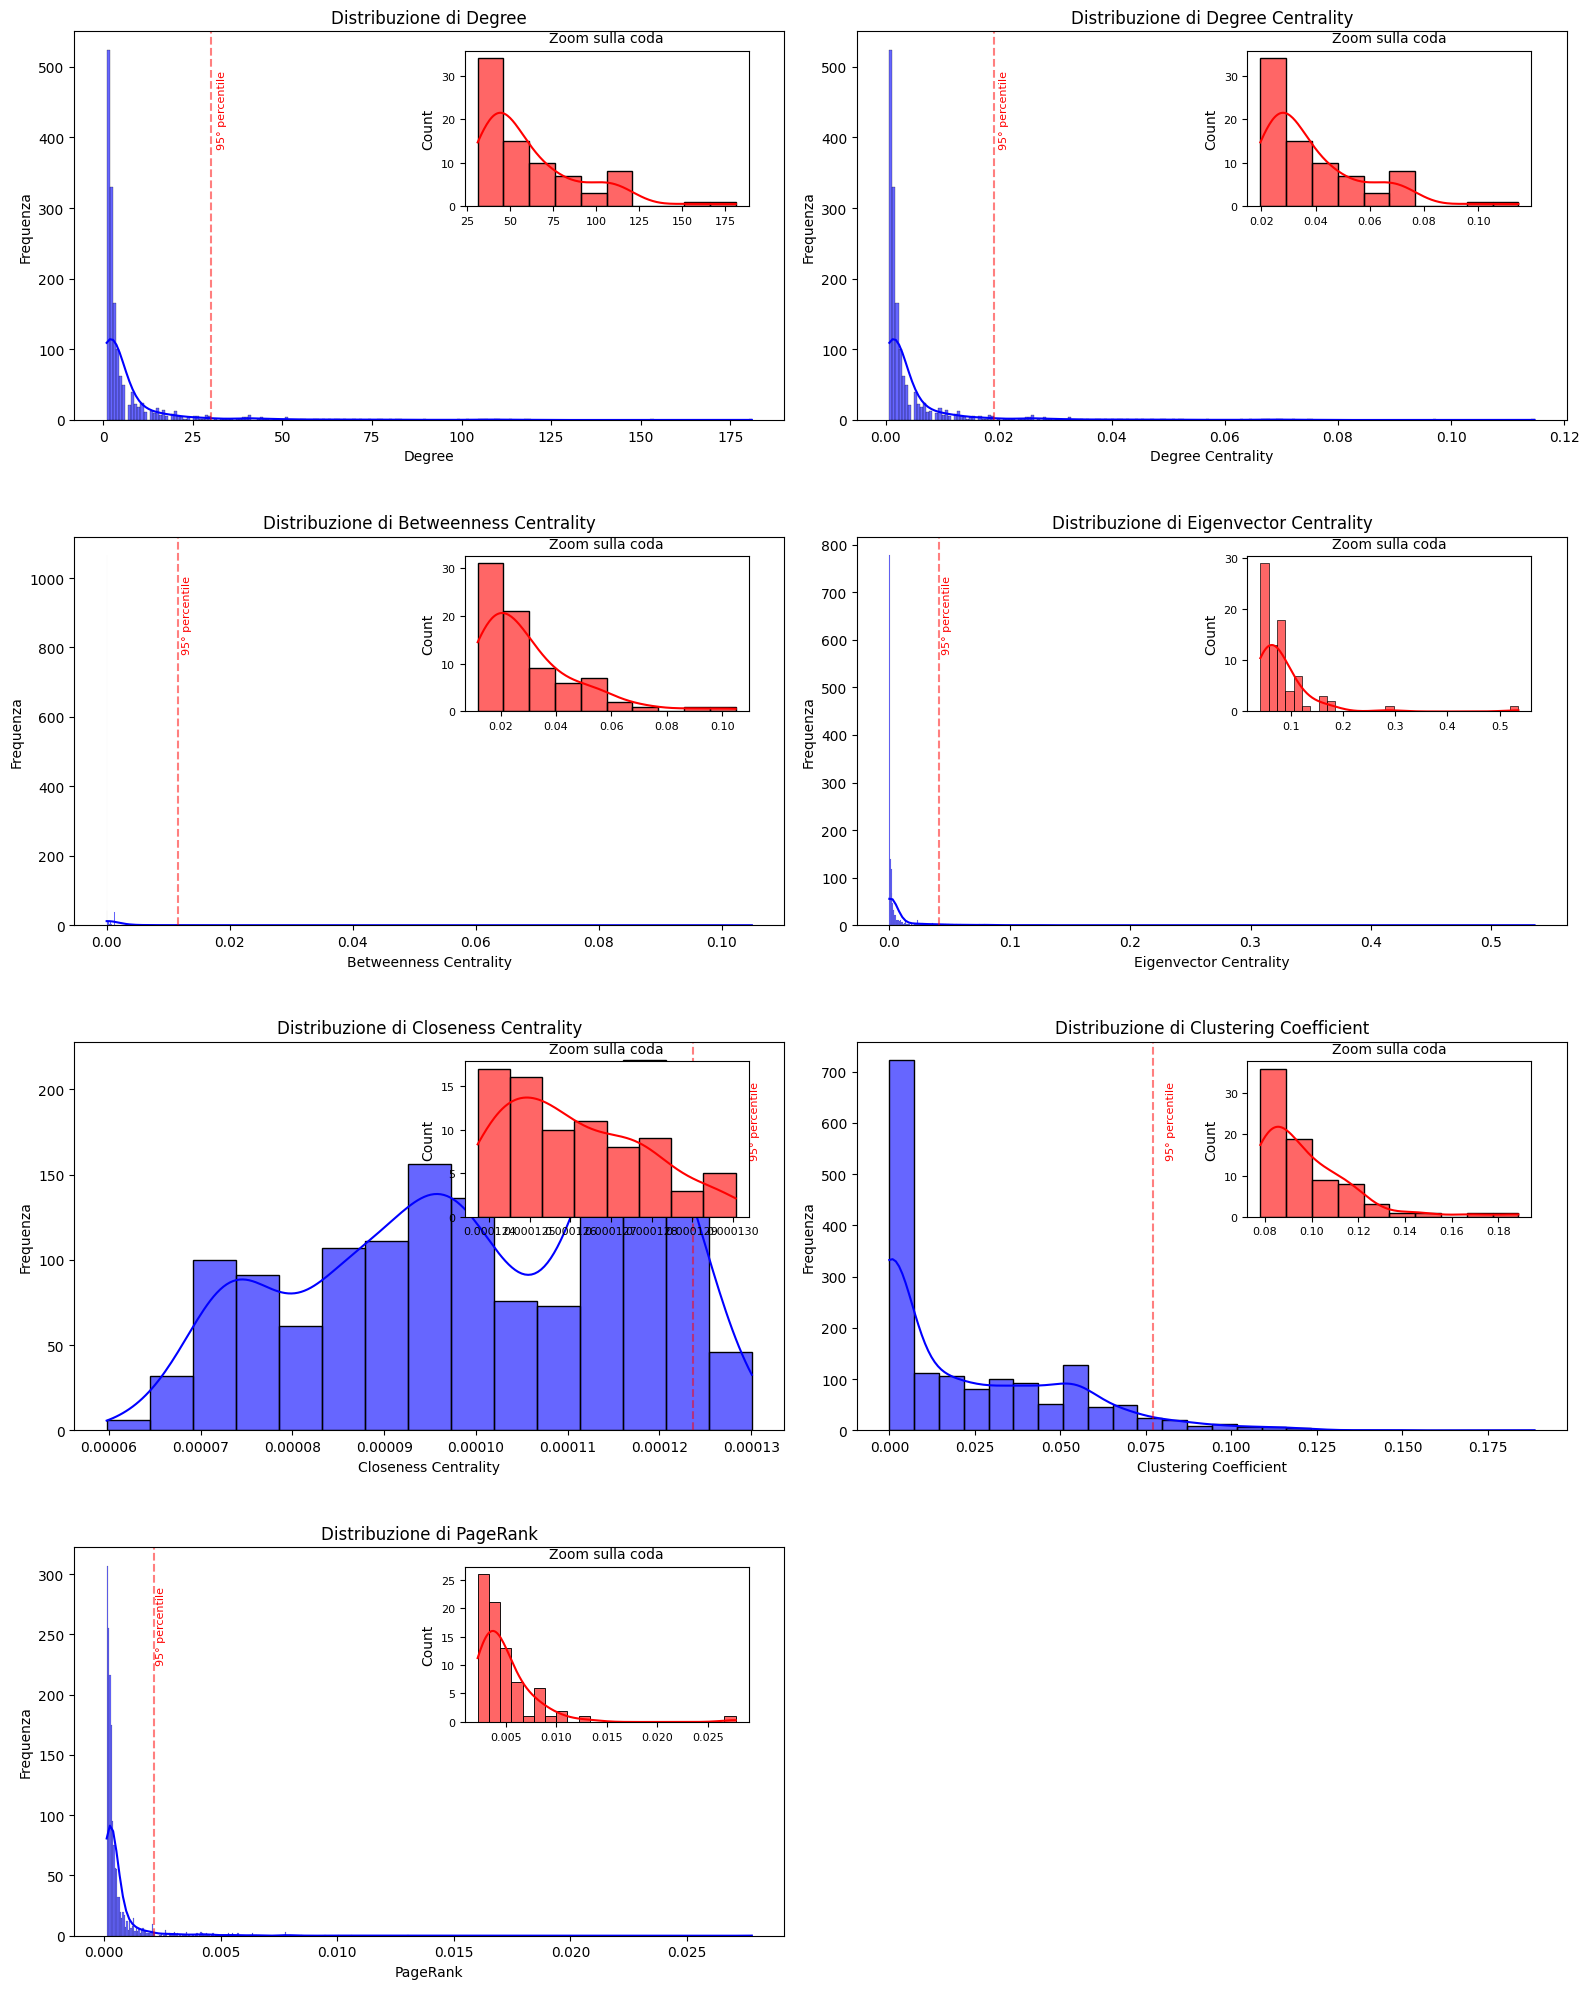
\includegraphics[width=0.8\linewidth]{img/distribution_queues.png}
        \caption{Queue distribution}
    \end{figure}
    Analysis of linear distributions with a focus on queues (Figure 5) allows us to examine in more detail the behavior of airports above the 95th percentile, i.e., those that are exceptionally central according to the different metrics.
    For Degree and Degree Centrality, the dashed red line (95th percentile) is around 25-30, highlighting that only 5 percent of airports have a significant number of direct connections. Zooms on the tails show a decreasing but consistent distribution down to values of 150-175, confirming the existence of highly connected global hubs such as those identified in section 5.2.1.
    Betweenness Centrality shows a more distributed tail than Degree, consistent with the observation in Section 5.2.2 that airports such as Dallas, Beijing, Amsterdam, Los Angeles, and Singapore have significantly higher values than others, functioning as crucial bridges in the global network.
    Eigenvector Centrality has a relatively short and steep tail, indicating an even greater concentration of influence in the major hubs identified in Section 5.2.6.
    Closeness Centrality shows a more uniform distribution in the tail, confirming what was reported in Section 5.2.3 about the stability of values for many airports. This suggests relatively uniform accessibility in the network of major global hubs.
    The Clustering Coefficient shows a significant tail with values as high as 0.18, consistent with the results in Section 5.2.4, where it is noted that smaller regional airports tend to have higher clustering coefficients than large international hubs.

    \subsection{Relationships between Degree Centrality Measures}
    \begin{figure}[H]
        \centering
        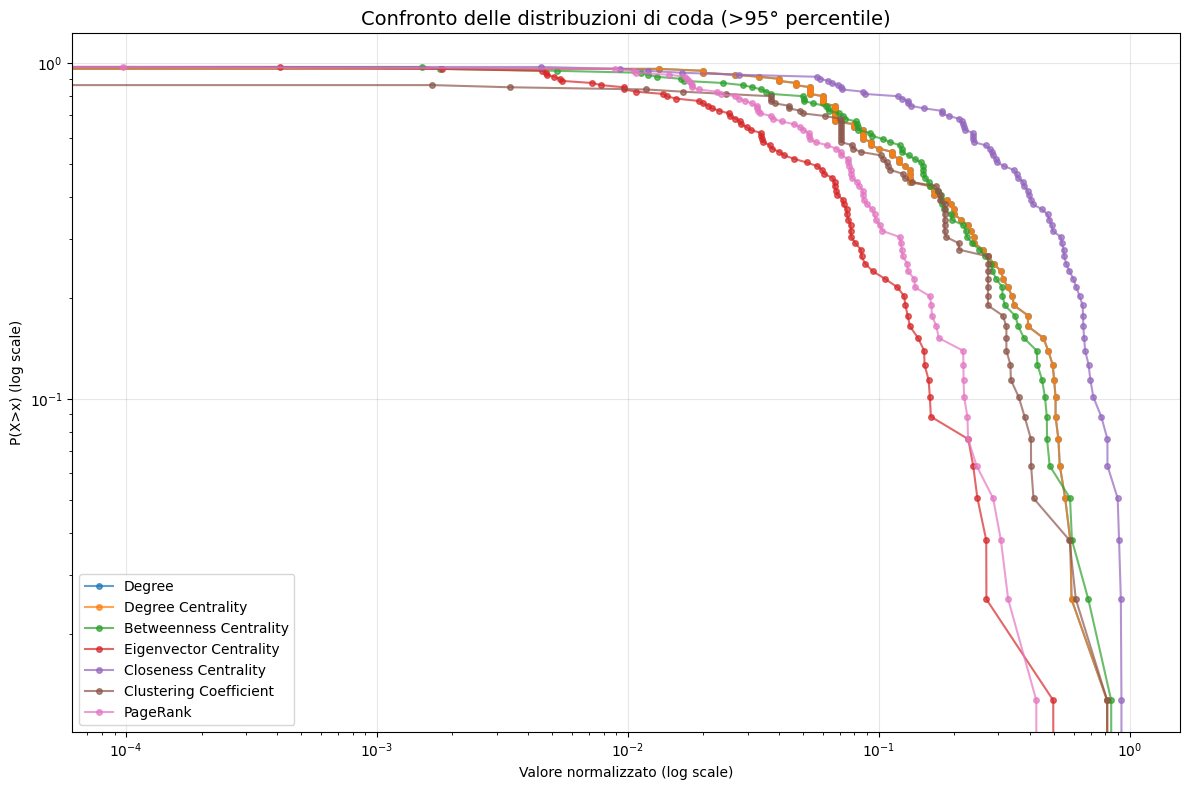
\includegraphics[width=0.8\linewidth]{img/relationships_between_degree_centrality_measures.png}
        \caption{Relationships between Degree Centrality Measures}
    \end{figure}
    Analysis of the relationships between Degree Centrality and other measures (Figure 6) reveals significant patterns in the structure of the global air network.
    The relationship between Degree Centrality and Betweenness shows a positive correlation but with significant dispersion. This confirms what was observed in Sections 5.2.1 and 5.2.2, where some Asian airports such as Beijing (PEK) and Singapore (SIN) have high betweenness despite not being in the top ranks for degree, highlighting their key role as intercontinental bridges.
    The correlation between Degree Centrality and Eigenvector is stronger, confirming the observation in section 5.2.6 that airports with higher degree also tend to be connected to other major hubs, reinforcing their crucial role in the network.
    The relationship between Degree Centrality and Closeness shows a weak but positive correlation, consistent with the relative homogeneity of closeness values found in section 5.2.3.
    The relationship between Degree Centrality and Clustering Coefficient is more complex and tends to be negative for high degree nodes, confirming what was observed in section 5.2.4, where smaller and regional airports tend to have higher clustering than large international hubs.
    
    \subsection{Correlations among Measures of Centrality.}
    \begin{figure}[H]
        \centering
        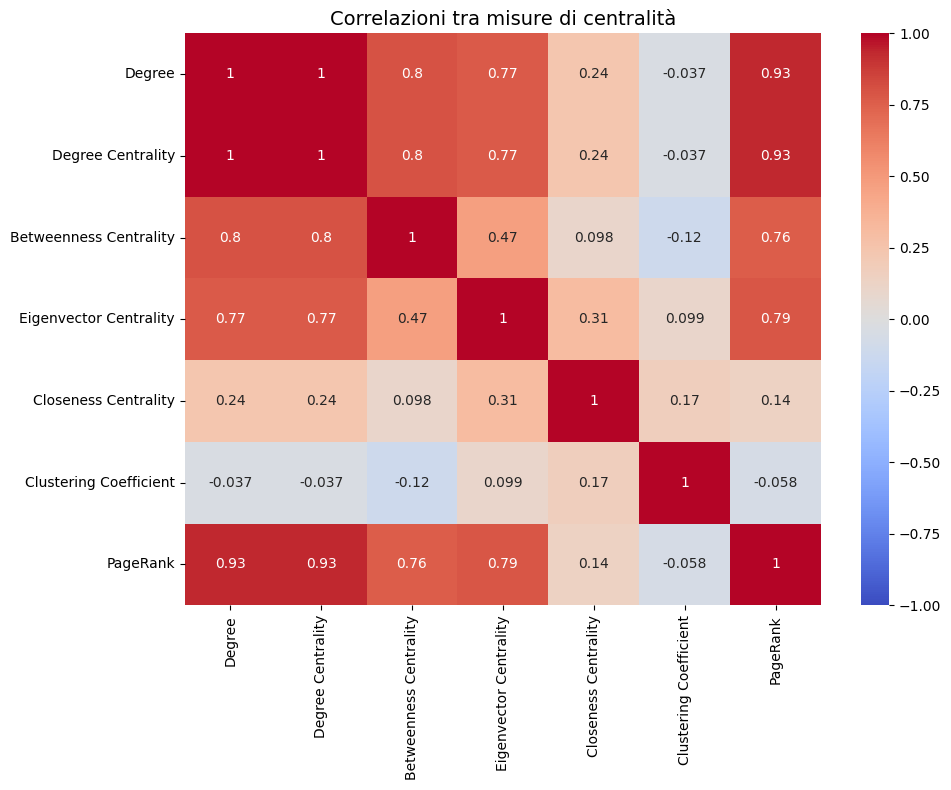
\includegraphics[width=0.8\linewidth]{img/correlations_measures_centrality.png}
        \caption{Correlations among Measures of Centrality.}
    \end{figure}
    The correlation matrix (Figure 7) quantifies the relationships between the different measures, providing a concise view of their interdependence.
    The strong correlation between Degree/Degree Centrality and PageRank (0.93) highlights how the number of direct connections is a determinant of an airport's overall importance in the network.
    The significant correlation between Degree/Degree Centrality and Betweenness (0.8) confirms what was discussed in Sections 5.2.1 and 5.2.2, where many of the airports with high Degree/Degree Centrality also appear among those with high betweenness, serving as both direct hubs and strategic bridges.
    The correlation between Degree/Degree Centrality and Eigenvector (0.77) supports what was observed in section 5.2.6, confirming that the most connected airports tend to be connected to other major airports.
    The moderate or weak correlations of Closeness Centrality with other measures reflect the homogeneity observed in section 5.2.3, indicating that this measure captures unique structural aspects of the network.
    The weak or slightly negative correlations of the Clustering Coefficient with other measures, particularly with Betweenness (-0.12), confirm what was discussed in section 5.2.4, where airports with high clustering tend to be regional nodes rather than global hubs.

    \subsection{Comparison of Tail Distributions}
    \begin{figure}[H]
        \centering
        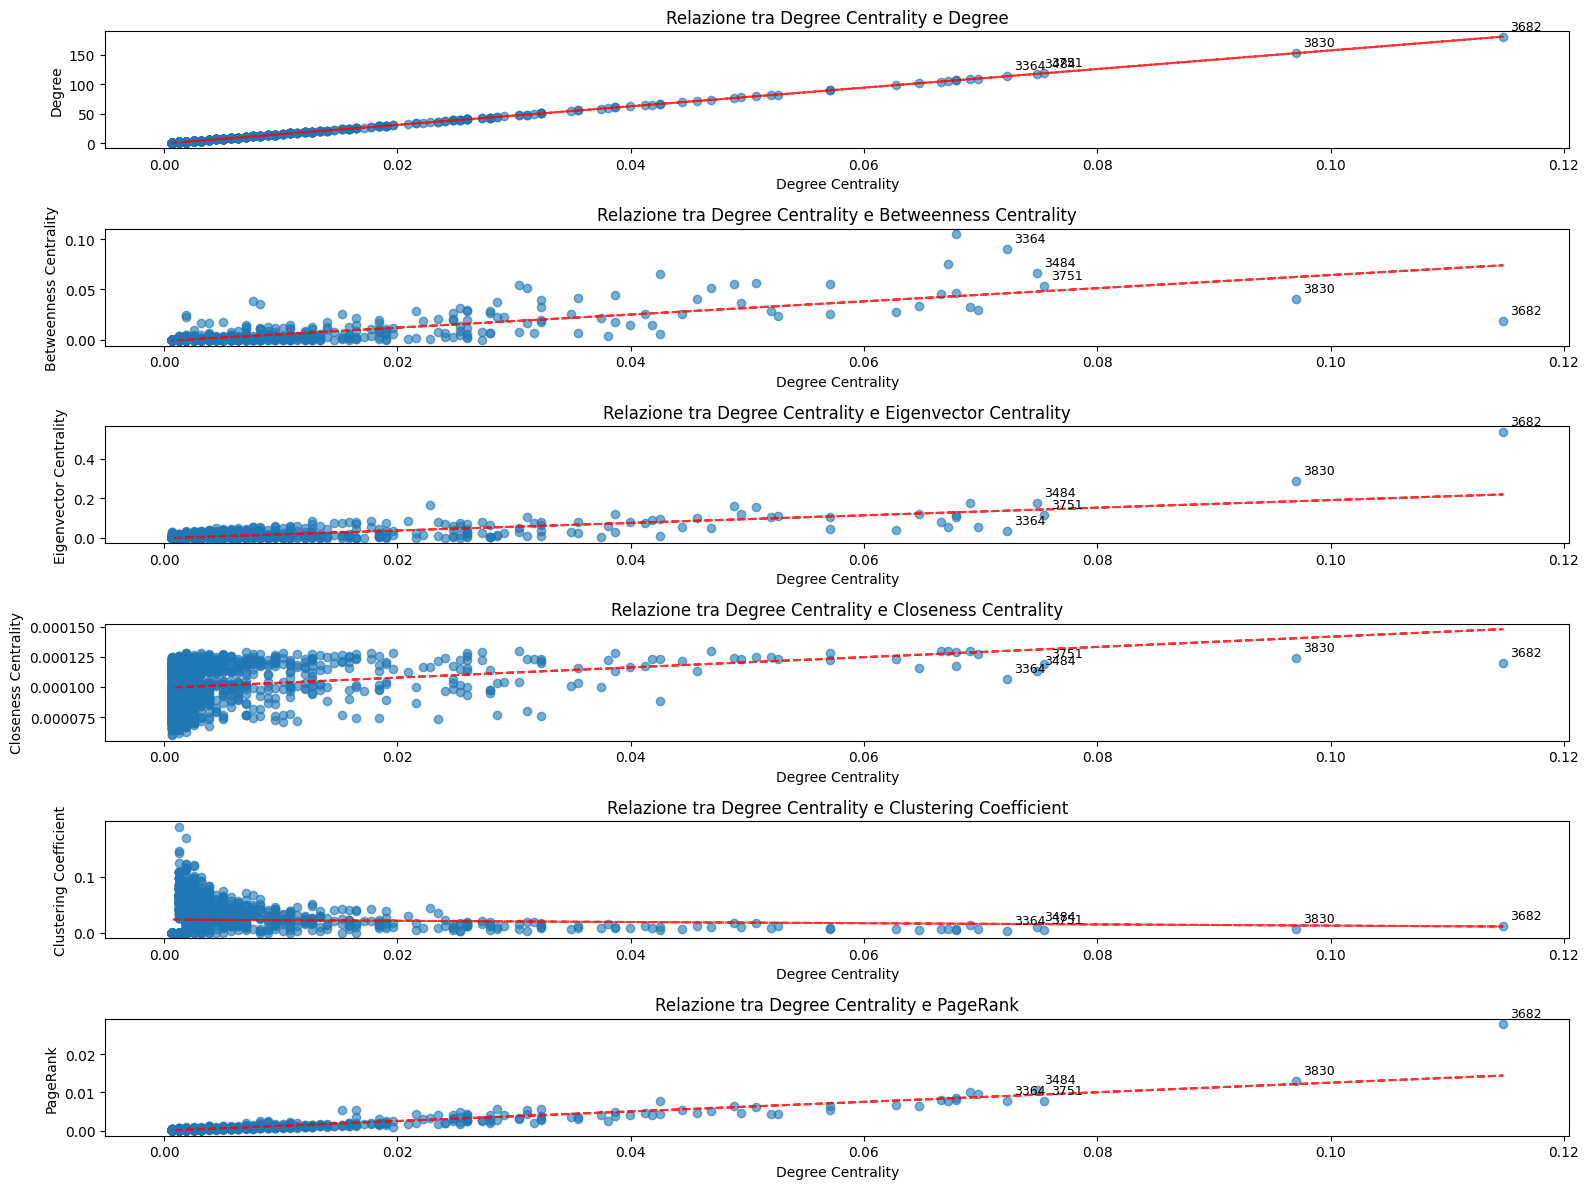
\includegraphics[width=0.8\linewidth]{img/tail_distribution.png}
        \caption{Correlations among Measures of Centrality.}
    \end{figure}
    Comparing the normalized tail distributions (Figure 8) allows us to assess the degree of inequality in the different measures of centrality for nodes above the 95th percentile.
    Eigenvector Centrality shows the fastest decay, indicating a less unequal distribution in the extreme values, consistent with the concentration of influence in the major hubs described in Section 5.2.6.
    Betweenness Centrality shows one of the heaviest tails, confirming what was discussed in section 5.2.2 about some airports serving as crucial bridges, with values significantly higher than others.
    Closeness Centrality shows the slowest decay, consistent with the homogeneity of values found in section 5.2.3.

    \subsection{Additional Metrics Description}\label{subsec:additional-metrics-description}

    \begin{itemize}
        \item \textbf{Average Path Length:} \texttt{10210.055112776308}

        This very high value likely reflects a weighted average, where the weights (distances in kilometers) are aggregated along paths. It indicates that, when considering these weights, the typical ``distance'' between airports is large. In contrast, the unweighted (hop-based) distances are much shorter.

        \item \textbf{Diameter of the Network:} \texttt{12}

        The diameter represents the maximum number of hops between any two airports. A diameter of 12 shows that, topologically, any airport can be reached from any other in no more than 12 steps, indicating a compact structure in terms of connectivity.

        \item \textbf{Number of Connected Components:} \texttt{1}

        This result confirms that the network is fully connected; every airport is reachable from any other, ensuring a unified air transport system.

        \item \textbf{Assortativity:} \texttt{-0.17902211456273712}

        The negative assortativity indicates a tendency for high-degree nodes (major hubs) to connect with low-degree nodes (smaller or regional airports). This disassortative mixing is typical in transportation networks, where central hubs connect to many less-connected nodes.

        \item \textbf{Number of Bridges:} \texttt{559}

        Bridges are edges whose removal would disconnect parts of the network. The presence of 559 bridges suggests that there are several critical routes whose loss could fragment the network, highlighting areas of potential vulnerability.
    \end{itemize}

    \subsubsection{Powerlaw}
    The power law fit yielded an exponent ($\alpha$) of approximately 1.8023. In a distribution of the form \( P(x) \propto x^{-\alpha} \), this value indicates a heavy-tailed behavior. Specifically, an exponent around 1.8 suggests that while many nodes (e.g., airports) have relatively few connections, a small number have extremely high connectivity. This pronounced heterogeneity implies that a few key hubs dominate the network structure, making them crucial for overall connectivity.

    \subsubsection{Clustering}
    Here is a representation of the clustering of the airports.

    \begin{figure}[H]
        \centering
        \includegraphics[width=1\linewidth]{img/community_clustering_graph}
    \end{figure}

    \subsection{Robustness}\label{subsec:robustness}
    The ability of the network to maintain a connection between all (or most) pairs of nodes when challenged. First, our team computed the first 10 hubs with the highest degree value. After that, we removed them from the network to check connectivity. The result was that we lost connectivity after the elimination of the hubs. Follow the fragmentation computation that resulted very low, so, the network is not fragmented. The third step is the computation of compactness. Initially, it was around \texttt{0.25}, but after removing the hubs, the network was not compact anymore.

    \subsubsection{Fragmentation Computation}
    Graph fragmentation assesses the structural integrity of a network by measuring how disconnected its components become when certain nodes are removed. To quantify this property, we used the following formula:
    
    \begin{equation}
        \text{Fragmentation} = 1 - \frac{\text{Size of largest connected component}}{\text{Total number of nodes in the graph}}
    \end{equation}
    
    We first computed the fragmentation of the original OpenFlights network, which yielded a value of 0. This indicates that the initial graph was completely connected, forming a single cohesive component where any airport could be reached from any other airport through a sequence of flights.
    
    Subsequently, we removed the top 10 hub airports (identified by their degree centrality) from the network and recalculated the fragmentation metric. After this targeted removal, the fragmentation value increased to 0.05, indicating that the network was no longer fully connected.
    
    This transition from 0 to 0.05 fragmentation has significant implications:
    
    \begin{itemize}
        \item \textbf{Loss of Network Cohesion:} The increase in fragmentation demonstrates that the graph is no longer compact. While 95\% of the airports still remain connected in the largest component, approximately 5\% have become isolated or form smaller disconnected clusters.
        
        \item \textbf{Hub Dependency:} This relatively modest intervention (removing just 10 nodes from a network containing hundreds of airports) resulted in a measurable fragmentation, highlighting the critical role these hub airports play in maintaining global connectivity.
        
        \item \textbf{Network Vulnerability:} The results reveal a structural vulnerability in the global air transportation network. The removal of key hubs creates isolated communities of airports that become unreachable from the main component.
        
        \item \textbf{Practical Consequences:} From a practical perspective, this means that certain regions or locations would become inaccessible via air travel if these major hub airports were unavailable, requiring alternative transportation methods or significant rerouting.
    \end{itemize}
    
    The analysis confirms the typical scale-free network property of the air transportation system, where a small number of highly connected nodes (hubs) are essential for maintaining the network's overall connectivity. This property creates efficiency in normal operations but introduces vulnerability to targeted disruptions affecting those hubs.
    
    This fragmentation analysis provides valuable insights for understanding network resilience and can inform strategic planning for transportation networks, disaster response, and infrastructure investment.
    \texttt{0.05}.

    \subsubsection{Compactness Computation}
    Graph compactness tells how "tightly" a graph is connected. The value for the original graph is \texttt{0.25}. After removing the top 10 hubs, the graph is no longer compact.

    \subsubsection{Centrality Analysis}
    At the end, we proceeded with the computation of the Betweenness Centrality. Then we visualized the most influenced airports about the new computation of the metric.

    \begin{figure}[H]
        \centering
        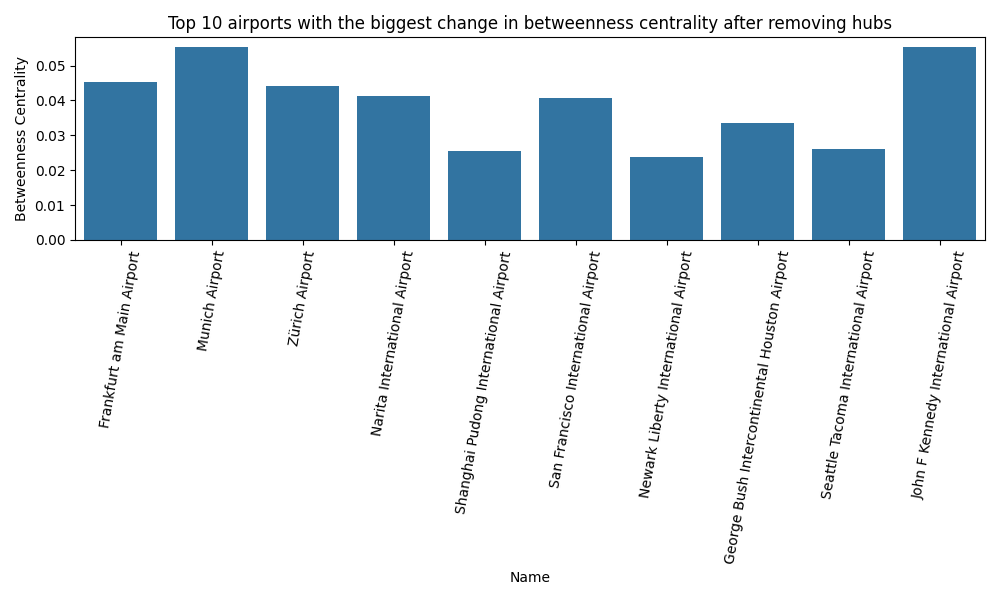
\includegraphics[width=0.8\linewidth]{img/biggest_changes_betweenness_centrality}
    \end{figure}
    Airports like \textbf{Munich} (MUC) and \textbf{New York Kennedy} (JFK) demonstrate the largest increases in betweenness centrality, with values exceeding 0.05. This substantial jump indicates that these airports rapidly assume critical bridging roles when main hubs are removed from the network. \\

    The data reveals a clear hierarchical pattern among these airports: the top tier (MUC, JFK) shows nearly twice the betweenness increase compared to the bottom tier (SEA, PVG, EWR). The middle tier consisting of \textbf{Frankfurt} (FRA), \textbf{Zurich} (ZRH), \textbf{Morristown} (MRT), and \textbf{San Francisco} (SFO) exhibits intermediate values between 0.041-0.045, positioning them as significant but not dominant secondary hubs. \\
    
    Notably, the geographic distribution shows a concentration of European airports (Munich, Frankfurt, Zurich) and North American facilities (JFK, SFO, IAH, SEA, EWR) among those gaining the most centrality. This suggests these regions maintain robust alternative routing capabilities when primary hubs are unavailable. \\
    
    These findings highlight the network's adaptive resilience: when major connection points are removed, these secondary airports rapidly increase their importance as transfer points, ensuring the network maintains functional connectivity, albeit potentially with less efficient routing. The significant increases in betweenness centrality demonstrate how the global air transportation network reconfigures its flow patterns to accommodate the loss of primary hubs. \\
    
    This analysis provides valuable insights for understanding network vulnerability and identifying which airports serve as critical backups in contingency scenarios. The airports showing the largest increases would be prime candidates for capacity expansion if network resilience is a priority for transportation planners.


    \section{Conclusions}\label{sec:conclusions}
    The conclusions of the study on the global air transport network highlight several critical insights derived from the analysis of airport connectivity and centrality measures. The project aimed to identify the most relevant and strategic airports that play a pivotal role in facilitating global connectivity. Through the application of various centrality metrics, including betweenness centrality, closeness centrality, eigenvector centrality, and PageRank, the research successfully pinpointed key airports that serve as vital nodes within the air transportation system.

    One of the primary findings of the study was the confirmation of the hypothesis that airports with high centrality between is essential to maintain global connectivity. These airports act as crucial bridges along the shortest routes between other airports, indicating their importance in linking different regions and facilitating efficient air travel. Robustness simulations conducted during the analysis demonstrated that the removal of these high-betweenness airports would lead to significant fragmentation and reduced connectivity within the network. This underscores the necessity of these airports in ensuring seamless air travel and highlights their strategic importance in the global transportation landscape.

    Additionally, the findings offer insights into the overall structure and dynamics of the air transport network. This information can improve route planning and air traffic management, helping airlines optimize operations, reduce costs, and enhance service. Moreover, understanding the role of major hubs aids in assessing network resilience to disruptions, ensuring the stability and reliability of air travel vital for economic growth and global mobility.
\end{document}